\documentclass{article}

% Package necessari
\usepackage[a4paper]{geometry}
\usepackage[utf8]{inputenc}
\usepackage[english]{babel}
\usepackage[T1]{fontenc}
\usepackage[font={small,sl}]{caption}
\usepackage[font={small,sl}]{subcaption}
\usepackage{graphicx}
\usepackage[usenames, table, dvipsnames]{xcolor}
\usepackage{hyperref}
\usepackage[most]{tcolorbox}
\usepackage[section]{placeins}
\usepackage{soulutf8}
\usepackage{listings}
\usepackage{tabularray}


% Titolo del documento
\title{\small Report of "Network \& System defense" project \\
\Huge \textbf{MLKM SHIELD}\\
\Large (Protection against malicious LKM)}

% Autore del documento
\author{Simone Tiberi (M. 0299908)\\%
(email: \texttt{\href{mailto:simone.tiberi.98@gmail.com}{simone.tiberi.98@gmail.com}})}

% Data del documento
\date{\today}

% Impostazione delle lunghezze di alcuni elementi del documento
\setlength{\parskip}{1em}
\setlength{\parindent}{0em}

% Impostazioni del package hyperref
\hypersetup{
        colorlinks=true,
        linktocpage=true,
        linkcolor=blue,
        urlcolor=blue,
        citecolor=blue,
        pdftitle={Relazione progetto NSD},
        pdfauthor={Simone Tiberi},
}

% Tokyonight colors
\definecolor{tn-bg}{HTML}{24283b}
\definecolor{tn-terminal}{HTML}{414868}
\definecolor{tn-red}{HTML}{f7768e}
\definecolor{tn-fg}{HTML}{c0caf5}
\definecolor{tn-fg-dark}{HTML}{a9b1d6}
\definecolor{tn-green}{HTML}{9ece6a}
\definecolor{tn-comment}{HTML}{565f89}
\definecolor{tn-blue0}{HTML}{3d59a1}
\definecolor{tn-blue}{HTML}{7aa2f7}
\definecolor{tn-cyan}{HTML}{7dcfff}

\lstset{
	language=C,
	frame=shadowbox,
        backgroundcolor=\color{tn-bg},
	rulesepcolor=\color{tn-terminal},
        basicstyle=\color{tn-fg}\ttfamily\scriptsize,
	keywordstyle=\color{tn-red}\bfseries\scriptsize,
	stringstyle=\color{tn-green}\scriptsize,
	commentstyle=\color{tn-comment}\scriptsize,
	numbers=left,
	numberstyle=\tiny\color{tn-fg-dark},
	numbersep=5pt,
	tabsize=2,
	showtabs=false,
	showspaces=false,
	showstringspaces=false,
	escapechar=|,
	captionpos=b,
	breaklines=true,
	keepspaces=true
}

\renewcommand{\lstlistingname}{Listato}
\graphicspath{ {./figs/} }

\newtcolorbox{custombox}[1]{
        colframe = blue!25,
        colback  = blue!10,
        coltitle = blue!20!black,
        title    = #1,
        breakable,
        enhanced,
}

\newcommand{\terminal}[1]{\colorbox{tn-bg}{\textcolor{tn-fg}{\texttt{#1}}}}

\begin{document}
\maketitle
	\section{Project specification}
	This project entails writing some protection mechanism in the Linux kernel (as a patch, a security
	module, a simple module, \dots) to prevent malicious loadable kernel modules to tamper with
	internal data structures of the kernel.

	In particular, beyond the example that we have discussed in class, it is possible that a module will
	not perform any attack during the loading phase, but it will perform some form of delayed attack
	(e.g., by relying on a Tasklet). Your scheme should also be able to perform this kind of detection.

	If a module is detected as malicious, it must be unmounted, and any possible side effect
	generated by it should be reverted.

	\section{Project structure}
	As can be seen in the Github repository~\cite{github:repo}, the project is organized into several
	files, each of which contains stuffs relating to certain components of the project (e.g. hooks,
	\textit{machine-specific} operations, \dots).

	The following sections are aimed at describing each component of the module developed, by analyzing
	core data structures and procedures implemented, as well as the general idea behind the
	functioning of the module.

	\section{Introduction to LKM monitoring}
	The protection mechanism is based on the assumption that when the shield module is mounted, the memory is
	in a \textit{good} state. As a matter of fact, in the beginning of the installation process the state of
	the critical memory areas is \textbf{cached}.

	Taking advantage of the \texttt{kretpobe} (and also \texttt{kprobe}) mechanisms offered by Linux
	Kernel~\cite{doc:kprobe} the very last function invoked by the kernel inside the mounting process
	is hooked, so that after the return statement, a \textbf{verification step} can begin
	(fig.~\ref{fig:monitoring}).

	\begin{figure}[!htbp]
		\centering
		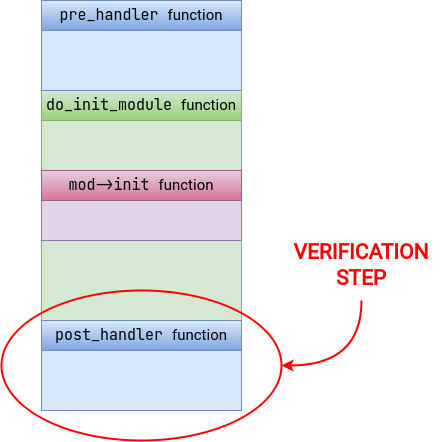
\includegraphics[scale=0.4]{monitoring}
		\caption{Hook scheme for \texttt{do\_init\_module}}
		\label{fig:monitoring}
	\end{figure}

	Obviously, using only this mechanism, a condition like the following one could occur:
	\begin{itemize}
		\item a non-malicious module $A$ is running a function $\alpha$,
		\item a malicious module $B$ is running \ul{concurrently} (such as shown in fig.~\ref{fig:concurrency}) a
		function $\beta$,
		\item the shield module recognize $A$ as malicious \ul{and also $B$ as non-malicious} thus \textbf{making two mistakes}.
	\end{itemize}

	\begin{figure}[!htbp]
		\centering
		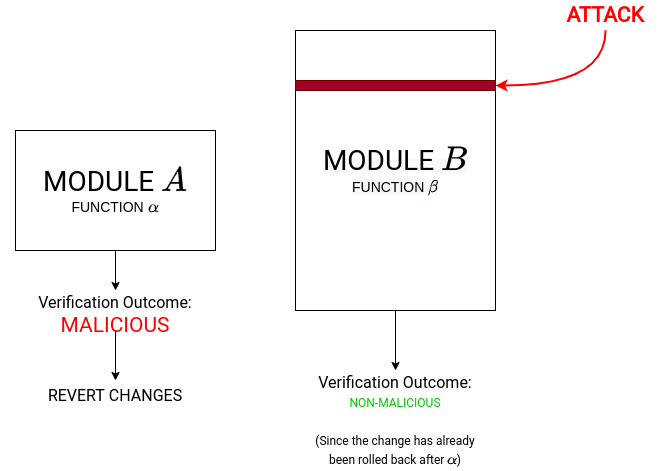
\includegraphics[scale=0.4]{concurrency}
		\caption{Detection scheme problem without using IPI}
		\label{fig:concurrency}
	\end{figure}

	For this reason the use of IPI has been introduced to ensure that:
	\begin{itemize}
		\item in the \textbf{pre-handler}, the core that is performing the mount (in an non-preemptible way) of the
		module, requires the others to spin on a certain barrier variable,
		\item in the \textbf{post-handler}, the same core as before changes the value of the barrier variable, thus
		allowing the restoration of normal activity.
	\end{itemize}

	Finally, for the detection of malicious actions in deferred mode, the probe mechanism was exploited again, this
	time dynamically hooking functions inside the module, as described in detail in the section ~\ref{sec:hooks}.

	\section{Components description}

	\bibliographystyle{plain}
	\bibliography{report}
\end{document}
